\section*{3.5}
%\addcontentsline{toc}{section}{Question 1}

a) On pose les conditions initiales suivantes :
\begin{align*}
    R = 1000\ \Omega,\ C = 100\cdot 10^{-6}\ \text{F},\ V = 110\sin(120\pi t),\ 
    v_c(0) = 0
\end{align*}

L'EDO à résoudre est :
\begin{align*}
    RCv_c' +v_c &= V \\
    0.1v_c' +v_c &= 110\sin(120\pi t) \\
    v_c' +10v_c &= 1100\sin(120\pi t)
\end{align*}

Le facteur intégrant est :
\begin{align*}
    \mu(t) = e^{\int{10}\ dt} = e^{10t}
\end{align*}

Ensuite, on trouve que la solution est :
\begin{align*}
    v_c(t) = Ce^{-10t} + e^{-10t}\int{1100\sin(120\pi t)\cdot e^{10t}\ dt}
\end{align*}

On intègre par parties :
\begin{table}[H]
    \centering
    %\caption{Mesures de tensions et de courants ainsi que le calcul du gain selon le courant $I_{\text{B}}$}
    \begin{tabular}{rrr}
	\toprule[1pt]
	 & D & I \\
	\midrule
	+ & $\sin(120\pi t)$ & $e^{10t}$\vspace{1mm}\\
	- & $120\pi\cos(120\pi t)$ & $0.1e^{10t}$\vspace{2mm}\\
	+ & $-(120\pi)^2\sin(120\pi t)$ & $0.01e^{10t}$\vspace{2mm}\\
	\bottomrule[1pt]
    \end{tabular}
\end{table}

Le résultat est :
\begin{align*}
    \int{\sin(120\pi t)e^{10t}\ dt} &= \f{1}{10}\sin(120\pi t)e^{10t}
    -\f{12}{10}\pi\cos(120\pi t)e^{10t}
    -\f{(120\pi)^2}{100}\int{\sin(120\pi t)e^{10t}\ dt} \\
    \int{\sin(120\pi t)e^{10t}\ dt} &= 7.031\cdot 10^{-5}\sin(120\pi t)e^{10t}
    -2.65\cdot 10^{-3}\cos(120\pi t)e^{10t}
\end{align*}

Finalement :
\begin{align*}
    v_c(t) &= Ce^{-10t} + 1100e^{-10t}\prt{7.031\cdot 10^{-5}\sin(120\pi t)e^{10t}
    -2.65\cdot 10^{-3}\cos(120\pi t)e^{10t}} \\
    v_c(t) &= Ce^{-10t} +7.73\cdot 10^{-2}\sin(120\pi t)
    -2.916\cos(120\pi t) \\
    v_c(t) &= Ce^{-10t} +2.9168\sin(120\pi t -1.544)
\end{align*}

Avec la condition initiale, on a :
\begin{align*}
    0 &= C +2.9168\sin(-1.544)\implies C = 2.9158
\end{align*}

La solution est :
\begin{align*}
    v_c(t) &= 2.9158e^{-10t} +2.9168\sin(120\pi t -1.544)
\end{align*}

b) L'expression du courant $i(t)$ est :
\begin{align*}
    i(t) &= Cv_c' = 100\cdot 10^{-6}\dv{}{t}
    (2.9158e^{-10t} +2.9168\sin(120\pi t -1.544)) \\
    &= 100\cdot 10^{-6}
    (-29.158e^{-10t} +120\pi\cdot 2.9168\cos(120\pi t -1.544)) \\
    &= (-0.02916e^{-10t} +1.0996\cos(120\pi t -1.544))
\end{align*}

c) En régime permanent, on voit que $2.9158e^{-10t}\to 0$ et que l'amplitude
va osciller entre $\pm 2.9168$ Volts. L'angle de phase est de -1.544 radians.
\vspace{5mm}

d) et e) En traçant le graphique, on sera en mesure de déterminer la tension
maximale :
\begin{center}
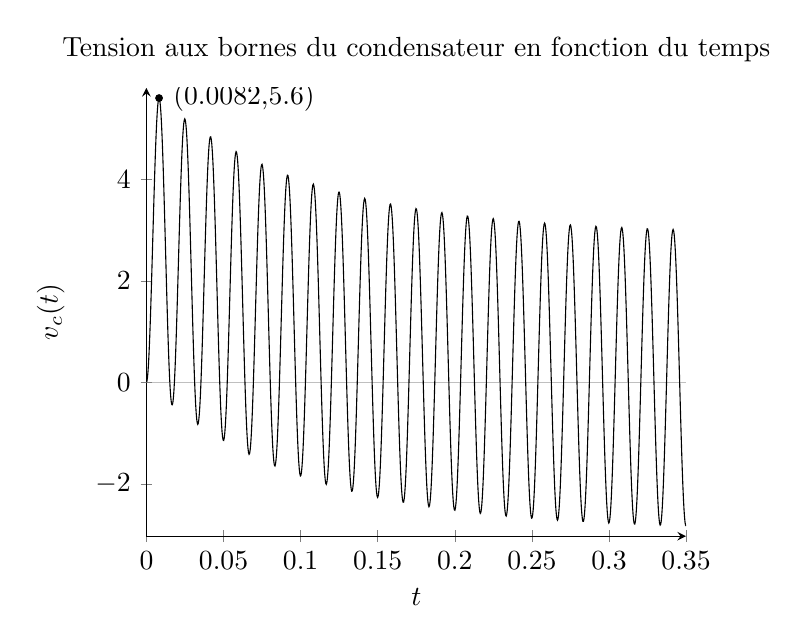
\begin{tikzpicture}
\begin{axis}[
    title = Tension aux bornes du condensateur en fonction du temps,
    extra y ticks       = 0,
    extra y tick labels = ,
    extra y tick style  = { grid = major },
    axis lines = left,
    xlabel = \(t\),
    ylabel = {\(v_c(t)\)},
    xticklabel style={/pgf/number format/fixed},
    enlarge y limits=0.024,
]
% Plot de la position
\addplot [
    domain=0:0.35, 
    samples=1000, 
    color=black,
] {2.9158*e^(-10*x) + 2.9168*sin(deg(120*pi*x-1.544))};
\node[label={0:{(0.0082,5.6)}},circle,fill,inner sep=1pt] at (axis cs:0.0082,5.6) {};
\end{axis}
\end{tikzpicture}
\end{center}

Sur le graphique, on voit la phase transitoire et le régime permanent. De plus,
le maximum local est localisé au temps $t=0.0082$ avec une tension de 5.6 V.
